\documentclass{beamer}					% Document class

\usepackage[english]{babel}				% Set language
\usepackage[utf8x]{inputenc}			% Set encoding
\usepackage{tikz}

\mode<presentation>						% Set options
{
  \usetheme{default}					% Set theme
  \usecolortheme{default} 				% Set colors
  \usefonttheme{default}  				% Set font theme
  \setbeamertemplate{caption}[numbered]	% Set caption to be numbered
}


\usepackage{graphicx}					% For including figures
\usepackage{booktabs}					% For table rules
\usepackage{hyperref}					% For cross-referencing

\title{Portfolio Rebalancing\\
with Reinforcement Learning}
\author{Deyu Zhang, Keyi Wang, Vedant Pathak, Felix Glombitza}								% Presentation author
\institute{FINM33165 Reinfocement and Deep Learning \\ University of Chicago}					% Author affiliation
\date{\today}									% Today's date	

\begin{document}


\begin{frame}
  \titlepage
\end{frame}

\begin{frame}{Outline}
  \tableofcontents
\end{frame}


\section{Methodology}

\begin{frame}{Literature Overview}
    
\end{frame}

\begin{frame}{Position of Project within Literature}
	\begin{figure}
	    \centering
	    \includegraphics[width=1\linewidth]{figures/plots_adjusted.png}
	    \caption{Existing literature on using Deep Reinforcement Learning in Trading. Minimally dapted from Millea(2021) for better readability.}
	    \label{fig:placeholder}
	\end{figure}
\end{frame}


\begin{frame}{Environment Diagram: General Case}
\begin{figure}[h!]
\centering
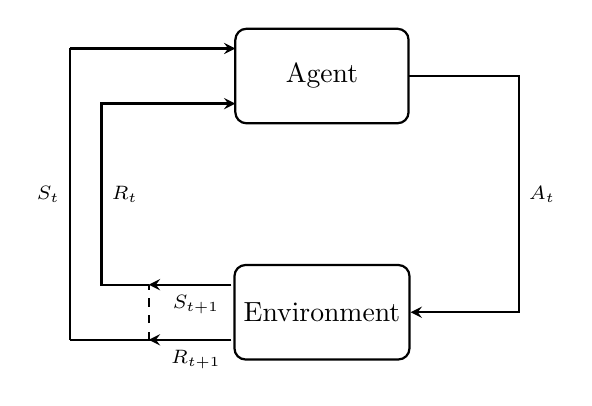
\begin{tikzpicture}[>=stealth, thick]

% ============================
% Nodes (NARROW WIDTH)
% ============================
\node[draw, rounded corners, minimum width=2.2cm, minimum height=1.2cm] (agent) at (0,0) {Agent};
\node[draw, rounded corners, minimum width=2.2cm, minimum height=1.2cm] (env)   at (0,-3) {Environment};

% Ports on Agent
\coordinate (Aupper) at (-1.1, 0.35);
\coordinate (Alower) at (-1.1,-0.35);

% Ports on Environment
\coordinate (Eupper) at (-1.15,-2.65);
\coordinate (Elower) at (-1.15,-3.35);

% Dashed line closer to boxes
\draw[dashed] (-2.2,-3.35) -- (-2.2,-2.65);

\coordinate (Dupper) at (-2.2,-2.65);
\coordinate (Dlower) at (-2.2,-3.35);

% ============================
% Right side: A_t
% ============================
\draw[->] (1.1,0) -- (2.5,0) -- (2.5,-3) -- (env.east);
\node[right] at (2.5,-1.5)
{\scriptsize
\textbf{$A_t$}
};

% ============================
% Outer left loop: S_t
% ============================
\draw[->] (-3.2,0.35) -- (Aupper);
\draw (-3.2,0.35) -- (-3.2,-3.35);
\draw[-] (-3.2,-3.35) -- (Elower);

\node[left] at (-3.2,-1.5)
{\scriptsize
\textbf{$S_t$}
};

% ============================
% Env → dashed arrows
% ============================
\draw[->] (Eupper) -- (-2.2,-2.65);
\node[below] at (-1.6,-2.65) {\scriptsize $S_{t+1}$};

\draw[->] (Elower) -- (-2.2,-3.35);
\node[below] at (-1.6,-3.35) {\scriptsize $R_{t+1}$};

% ============================
% Dashed → Agent (rectangular turn)
% ============================
\draw[->]
    (Dupper) -- (-2.8,-2.65)
             -- (-2.8,-0.35)
             -- (Alower);

% R_t label
\node[right] at (-2.8,-1.5)
{\scriptsize
\textbf{$R_t$}
};

\end{tikzpicture}
\end{figure}
\end{frame}


\begin{frame}{Environment Diagram: Portfolio Rebalancing}
\begin{figure}[h!]
\centering
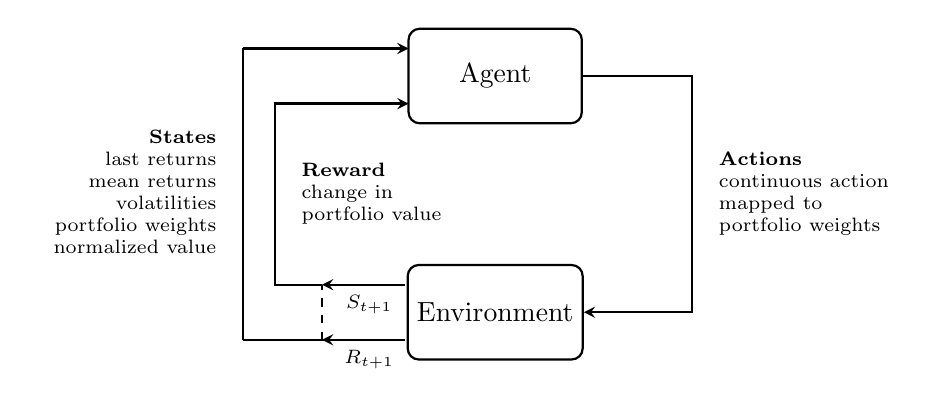
\begin{tikzpicture}[>=stealth, thick]

% ============================
% Nodes (NARROWER WIDTH)
% ============================
\node[draw, rounded corners, minimum width=2.2cm, minimum height=1.2cm] (agent) at (0,0) {Agent};
\node[draw, rounded corners, minimum width=2.2cm, minimum height=1.2cm] (env)   at (0,-3) {Environment};

% Ports on Agent
\coordinate (Aupper) at (-1.1, 0.35);
\coordinate (Alower) at (-1.1,-0.35);

% Ports on Environment
\coordinate (Eupper) at (-1.15,-2.65);
\coordinate (Elower) at (-1.15,-3.35);

% Dashed line closer to boxes
\draw[dashed] (-2.2,-3.35) -- (-2.2,-2.65);

\coordinate (Dupper) at (-2.2,-2.65);
\coordinate (Dlower) at (-2.2,-3.35);

% ============================
% Right side: ACTIONS (LEFT aligned)
% ============================
\draw[->] (1.1,0) -- (2.5,0) -- (2.5,-3) -- (env.east);
\node[right] at (2.5,-1.5)
{\scriptsize
\begin{tabular}{l}
\textbf{Actions} \\
continuous action \\
mapped to \\
portfolio weights
\end{tabular}
};

% ============================
% Outer left loop: STATES (RIGHT aligned)
% ============================
\draw[->] (-3.2,0.35) -- (Aupper);
\draw (-3.2,0.35) -- (-3.2,-3.35);
\draw[-] (-3.2,-3.35) -- (Elower);

\node[left] at (-3.2,-1.5)
{\scriptsize
\begin{tabular}{r}
\textbf{States} \\
last returns \\
mean returns \\
volatilities \\
portfolio weights \\
normalized value
\end{tabular}
};

% ============================
% Env → dashed arrows (short)
% ============================
\draw[->] (Eupper) -- (-2.2,-2.65);
\node[below] at (-1.6,-2.65) {\scriptsize $S_{t+1}$};

\draw[->] (Elower) -- (-2.2,-3.35);
\node[below] at (-1.6,-3.35) {\scriptsize $R_{t+1}$};

% ============================
% Dashed → Agent (rectangular turn)
% ============================
\draw[->]
    (Dupper) -- (-2.8,-2.65)
             -- (-2.8,-0.35)
             -- (Alower);

% Reward label (LEFT aligned)
\node[right] at (-2.8,-1.5)
{\scriptsize
\begin{tabular}{l}
\textbf{Reward} \\
change in \\
portfolio value
\end{tabular}
};

\end{tikzpicture}
\end{figure}
\end{frame}

\begin{frame}{Model}
	\begin{columns}
		\column{.5\textwidth}
        Text goes in first column.
        
        \column{.5\textwidth}
        Text goes in second column
	\end{columns}
\end{frame}

\section{Results}

\begin{frame}{Results}
	\input{tables/table1.tex}
\end{frame}


\begin{frame}{Evaluation}

\end{frame}

\begin{frame}{Conclusion and Outlook}
RL performs \textbf{profitably, but inconsistently}: inherent to the data, but also due to restrictions in approach
\vspace{\baselineskip}
    \begin{itemize}
        \item \textbf{State space:} price predictions, technical indicators
        \item \textbf{Action space:} more granular weights, more/different assets 
        \item \textbf{Rewards:} transaction costs, risk penalties
        \item \textbf{Model:} ensemble critics, attention-based networks
    \end{itemize}
\end{frame}

\nocite{*}

\begin{frame}{References}
  \small
  \bibliographystyle{apalike}
  \bibliography{references}
\end{frame}

\end{document}
